\documentclass[a4paper,papersize,dvipdfmx]{jsarticle}
\usepackage{ascmac}
\usepackage{mathtools, amssymb,bm}
\usepackage{comment}
\usepackage[hiresbb]{graphicx}
\usepackage{tcolorbox,color}
\usepackage{here}
\tcbuselibrary{raster,skins,breakable}

\newcommand{\pic}[1]{\begin{center} \includegraphics[width=1.0\linewidth,clip]{#1} \end{center}}   %写真用
\newcommand{\pict}[2]{\begin{center} \includegraphics[width= {#2} cm]{#1} \end{center}}   %写真用
\newcommand{\redunderline}[1]{\textcolor{red}{\underline{¥textcolor{black}{#1}}}}   %赤いアンダーライン
\newcommand{\mon}[1]{\item[({#1})] \ }
\newcommand{\ctext}[1]{\raise0.2ex\hbox{\textcircled{\scriptsize{#1}}}}%文字を丸囲みする(2桁の数字までならいける)

% 画像を貼る時はjpgかjpegで、pngはうまくいかないっぽい

%\itemを四角で囲った数字にする場合は以下のコメントアウトを消す
%\renewcommand{\labelenumi}{\textbf{\framebox[1.5zw]{\theenumi}}}


%enumerateの2階層めのカウンタを1,2,3, にする時は以下のコメントアウトを消す
\renewcommand{\theenumii}{\arabic{enumii}}

%enumerateのカウンタについては以下を参照
% http://www3.otani.ac.jp/fkdsemi/pLaTeX_manual/kajyo.html


%enumerateの番号の出力形式を変更するには、カウンタの値を出力する命令を定義し直す。
%レベル	カウンタ	出力する命令	デフォルトの出力
%1	enumi	¥theenumi	アラビア数字(1,2,3,・・・)
%2	enumii	¥theenumii	小文字のアルファベット(a,b,c,・・・)
%3	enumiii	¥theenumiii	小文字のローマ数字(小文字のローマ数字(\UTF{2170},\UTF{2171},\UTF{2172},・・・)
%4	enumiv	¥theenumiv	大文字のアルファベット(A,B,C,・・・)
%例:¥enumiカウンタを大文字のローマ数字で出力する設定
% ¥renewcommand{¥theenumi}{¥Roman{enumi}}

% 番号の出力形式
%命令	出力形式
%¥arabic	アラビア数字(1、2、3、・・・)
%¥roman	ローマ数字(\UTF{2170}、\UTF{2171}、\UTF{2172}、・・・)
%¥Roman	ローマ数字(\UTF{2160}、\UTF{2161}、\UTF{2162}、・・・)
%¥alph	アルファベット(a、b、c、・・・)
%¥Alph	アルファベット(A、B、C、・・・)




\begin{document}

\title{実習レポート 有機合成化学教室}
\author{10191043 鈴木健一}
%作成日を入れる場合は消す
\date{}
\maketitle

%以下の3つからフォントサイズを選択するとよい
%\footnotesize
%\small
%\normalsize

\begin{flushright}
実験日 : 2019/5/20 $\sim$ 2019/5/27

共同実験者 : 白井孝平
\end{flushright}

\section*{1日目 トリクロロエチルエステル化}
\subsection*{結果}
\begin{itemize}
\item ナスフラスコ内にペニシリンGナトリウム塩、ピリジン、アセトン、2,2,2-Trichloroethyl chloroformateを加えて撹拌すると大量の泡が発生するのが確認された。


\end{itemize}
\subsection*{考察}
\begin{itemize}
\item 発生した泡は二酸化炭素であると考えられる。
\item 溶液が白くなった班と赤くなった班が出現したが、これはナトリウム塩とカリウム塩による違いらしい。


\end{itemize}
\section*{2日目 トリクロロエチルエステル化後処理、再結晶+Sの酸化仕込み}
\subsection*{結果}
\begin{itemize}
\item セライト濾過をした後の濾液と115 mLの水を加えると白い濁りが見え始めた。その後撹拌しながら放冷すると溶液全体が白く濁った。

\end{itemize}
\subsubsection*{TLC}
\begin{figure}[H]
\begin{center}
\begin{tabular}{c}

\begin{minipage}{0.22\hsize}
\begin{center}
\includegraphics[clip, width=4cm]{imgs2/tlc1.jpg}
\hspace{1.6cm} UV
\end{center}
\end{minipage}

\begin{minipage}{0.05\hsize}
        \hspace{2mm}
      \end{minipage}

\begin{minipage}{0.22\hsize}
\begin{center}
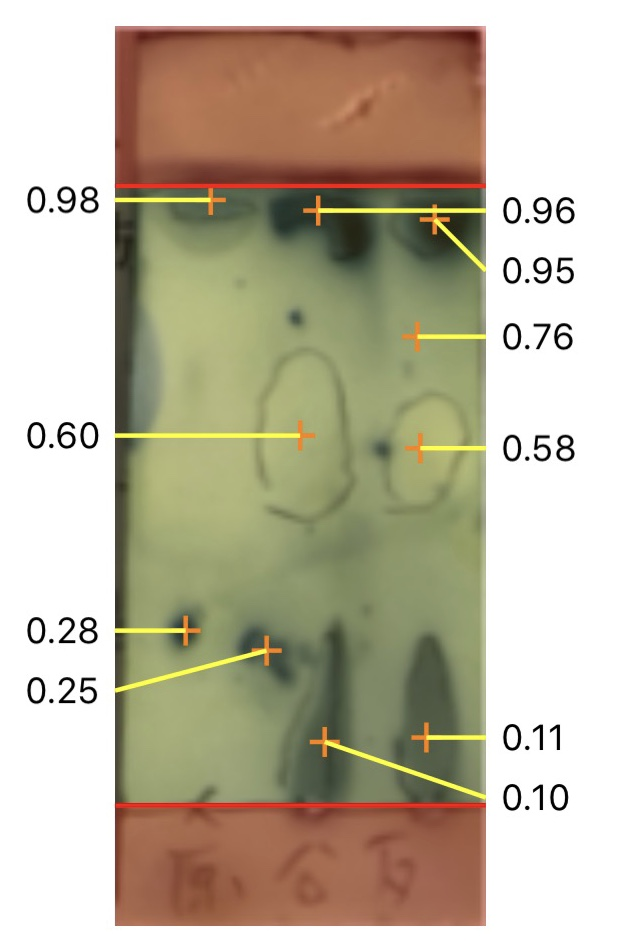
\includegraphics[clip, width=4cm]{imgs2/tlc2.jpg}
\hspace{1.6cm} リンモリブデン酸
\end{center}
\end{minipage}

\end{tabular}
\end{center}
\end{figure}

\subsubsection*{結晶}
\begin{itemize}
\item 形状・色 : 実習書には鱗片状の淡黄色の結晶が得られると書いてあったが、実際に得られたのは白色の粉末状の結晶だった。
\item 融点 : 141℃
\item 重さ : 8.51 g
\item 収率 : 63 $\%$

\end{itemize}
\section*{3日目 Sの酸化・後処理}
\subsection*{結果}
\begin{itemize}
\item エバポレーターで溶液を濃縮したとき、溶媒のほとんどが なくなった頃に白い結晶が析出した。
\item その後結晶をジクロロメタンに溶かし水浴で温めながらヘキサンを加えると再び白い結晶が析出した。
\item エタノールで再結晶すると白色の針状の結晶が得られた。

\end{itemize}
\subsubsection*{TLC}

\begin{figure}[H]
\begin{center}
\begin{tabular}{c}

\begin{minipage}{0.22\hsize}
\begin{center}
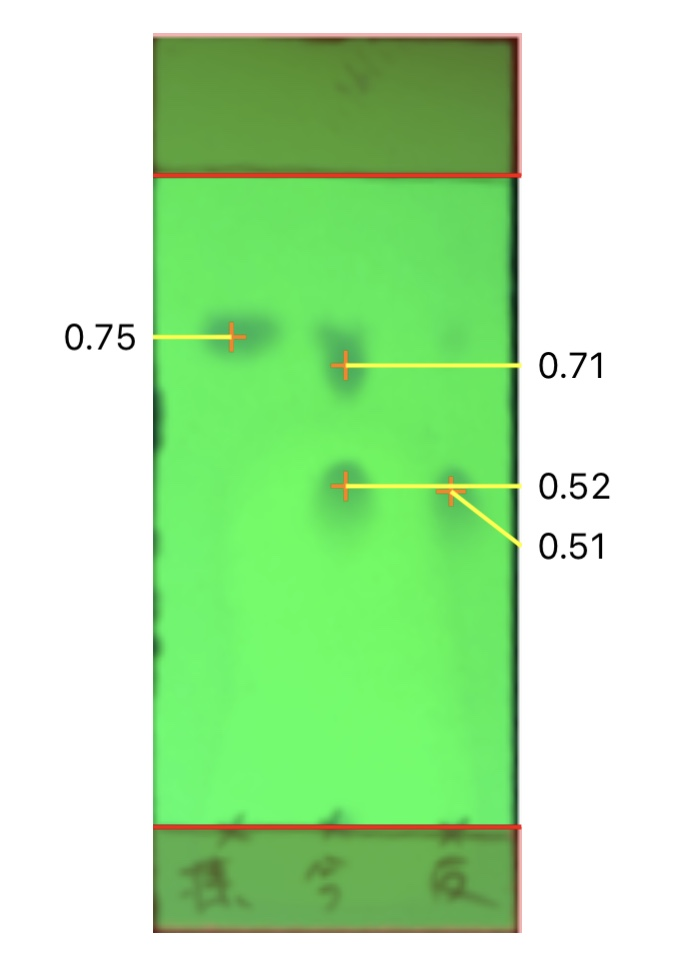
\includegraphics[clip, width=4cm]{imgs3/tlc1.jpg}
\hspace{1.6cm} UV
\end{center}
\end{minipage}

\begin{minipage}{0.05\hsize}
        \hspace{2mm}
      \end{minipage}

\begin{minipage}{0.22\hsize}
\begin{center}
\includegraphics[clip, width=4cm]{imgs3/tlc2.jpg}
\hspace{1.6cm} リンモリブデン酸
\end{center}
\end{minipage}

\end{tabular}
\end{center}
\end{figure}

\subsubsection*{再結晶}
\begin{itemize}
\item 重さ : 4.54 g
\item 収率 : 54.7 $\%$
\item 融点 : 158℃  ... 融点を測定すると画像のように色が変化した。

\pict{imgs3/yuten.jpg}{3}


\end{itemize}
\section*{4日目 環拡大}
\subsection*{結果}

\subsubsection*{反応}
ペニシリンGスルホキシド誘導体をDMFに溶解させ、無水酢酸を加えて油浴内で60分間加熱した。初めは無色透明だったがある時突然溶液の色が褐色に変わった。

\subsubsection*{分液操作}
反応液を10$\%$NaCl水に注ぎ、$\rm AcOEt / ether = 1/1$で抽出操作をおこなった。はじめは水層に溶けていた生成物が次第に有機層へと移っていくことが色の変化で確認された。

\begin{figure}[H]
\begin{center}
\begin{tabular}{c}


\begin{minipage}{0.20\hsize}
\begin{center}
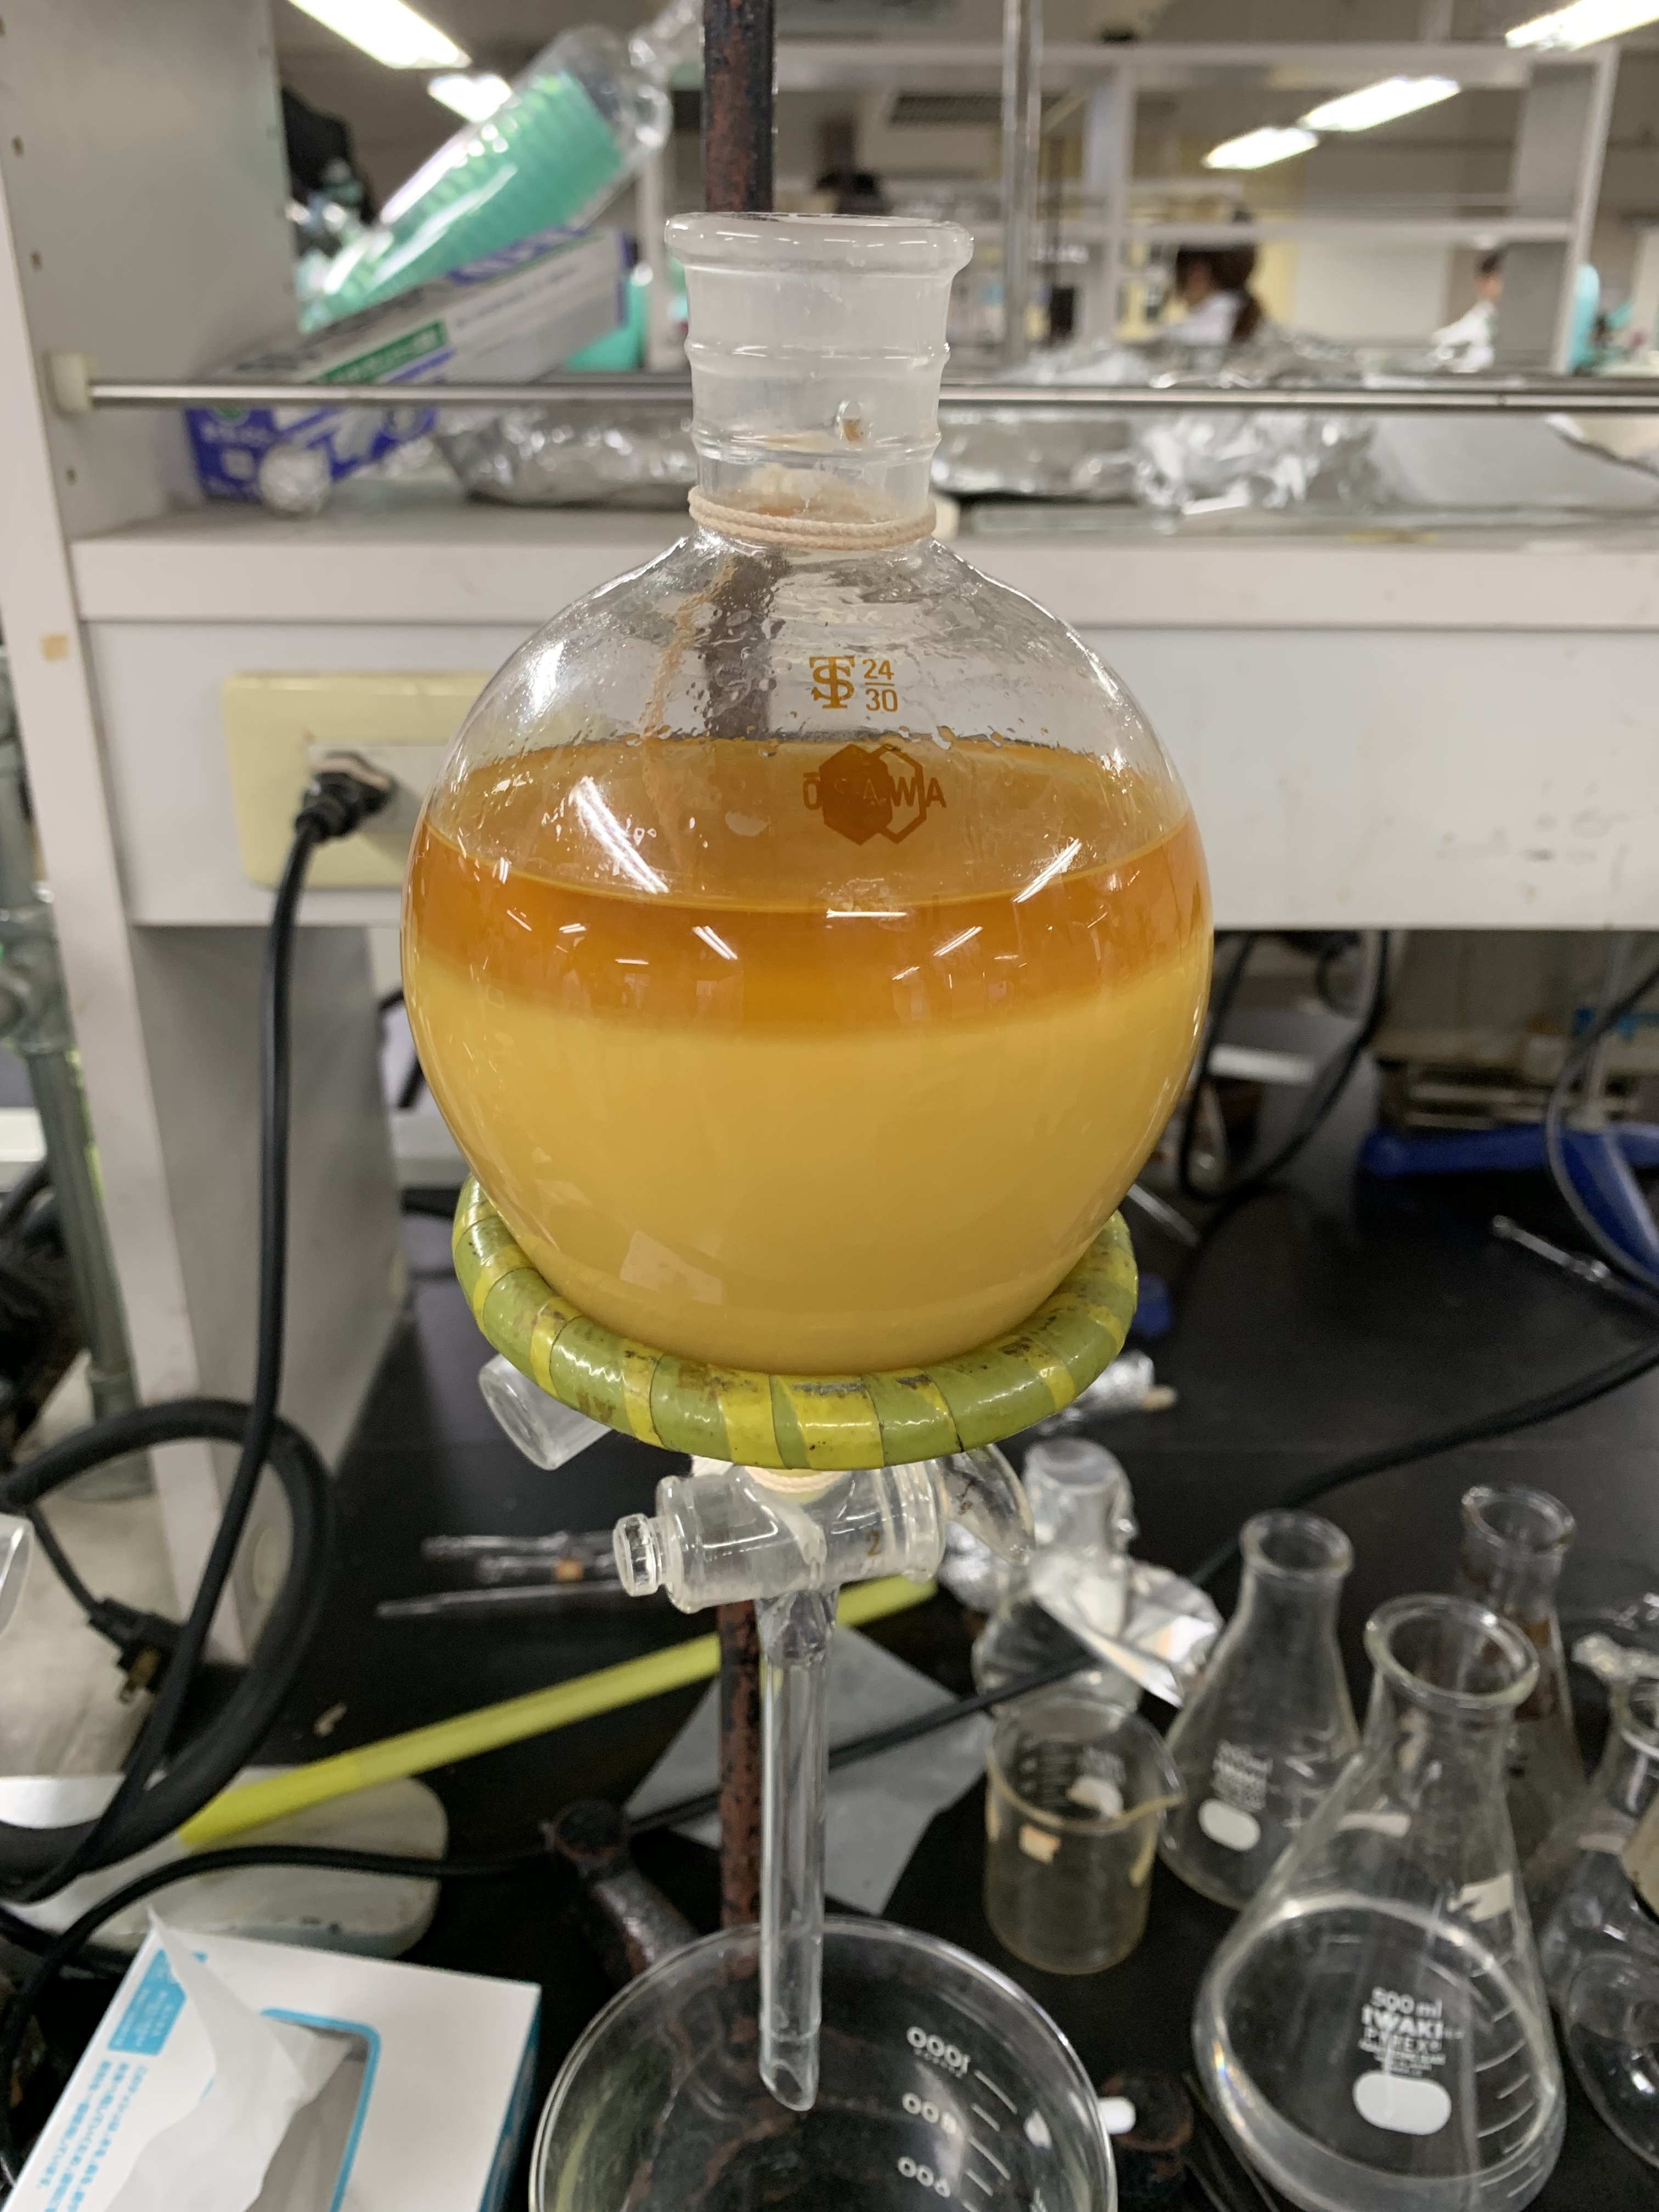
\includegraphics[clip, width=4cm]{imgs4/be1.jpg}
\hspace{1.6cm} 分液1回目 混ぜる前
\end{center}
\end{minipage}

\begin{minipage}{0.05\hsize}
        \hspace{2mm}
      \end{minipage}

\begin{minipage}{0.20\hsize}
\begin{center}
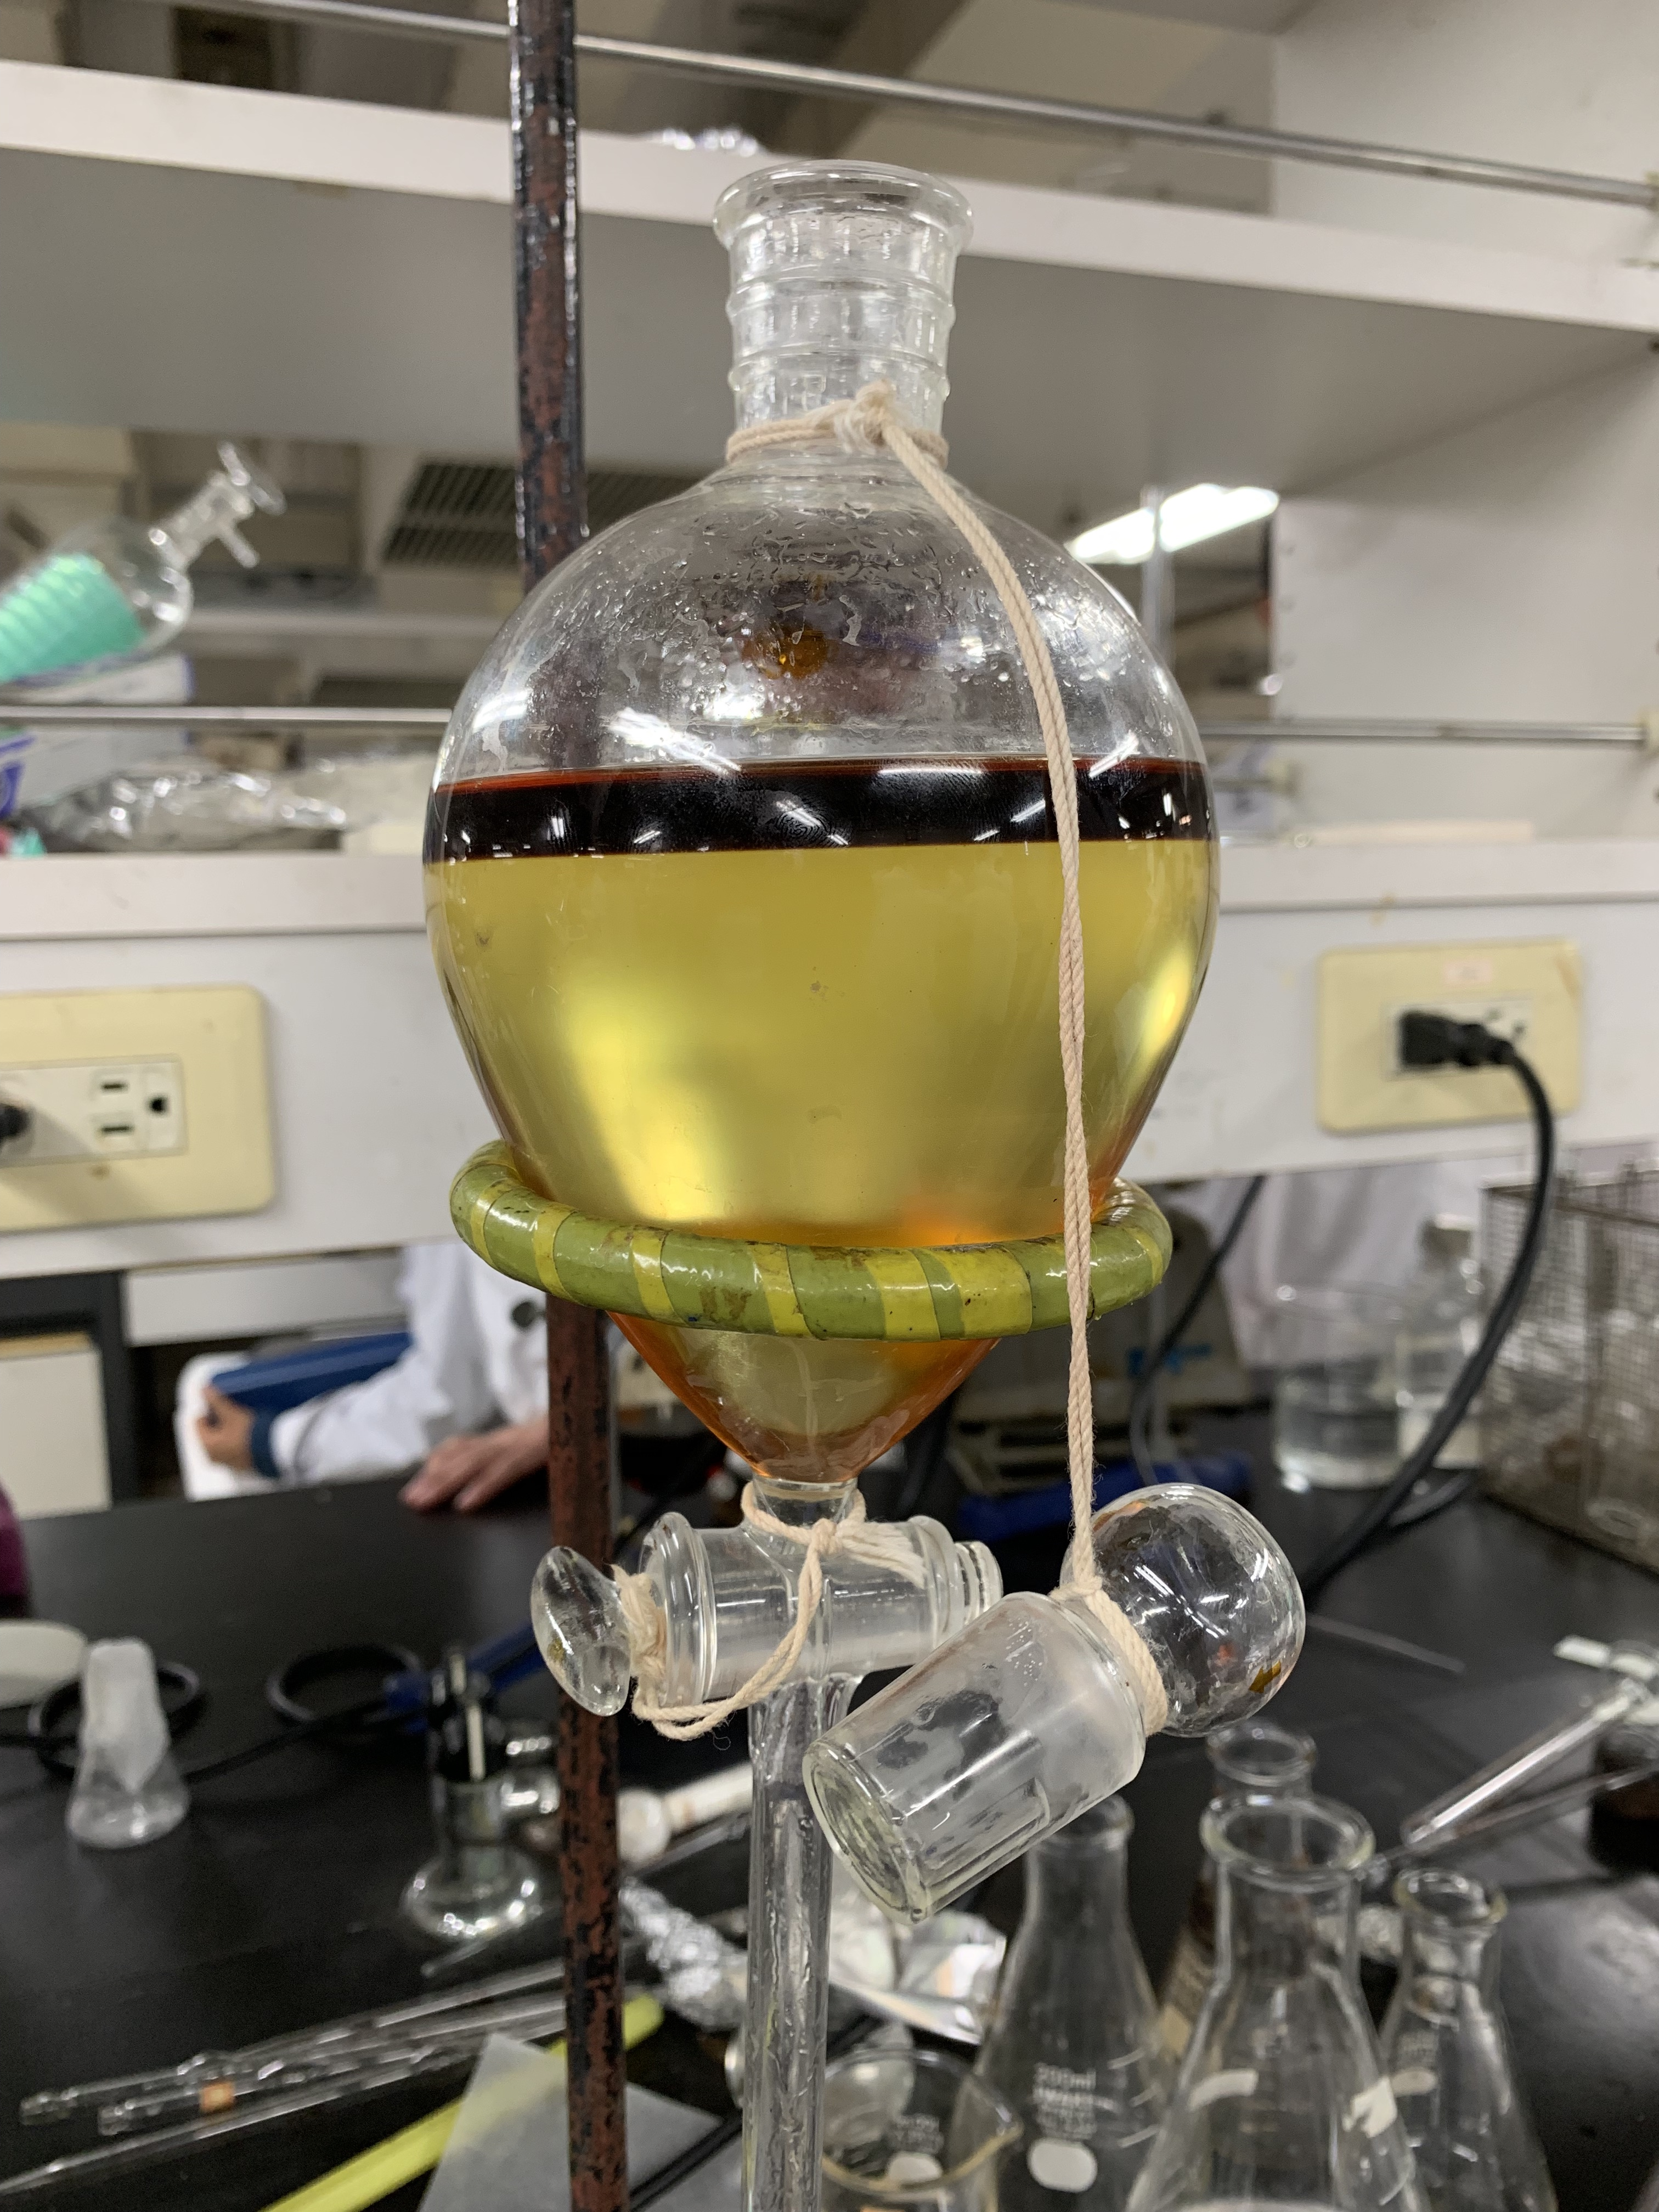
\includegraphics[clip, width=4cm]{imgs4/be2.jpg}
\hspace{1.6cm} 分液1回目 混ぜた後
\end{center}
\end{minipage}

\begin{minipage}{0.05\hsize}
        \hspace{2mm}
      \end{minipage}

\begin{minipage}{0.20\hsize}
\begin{center}
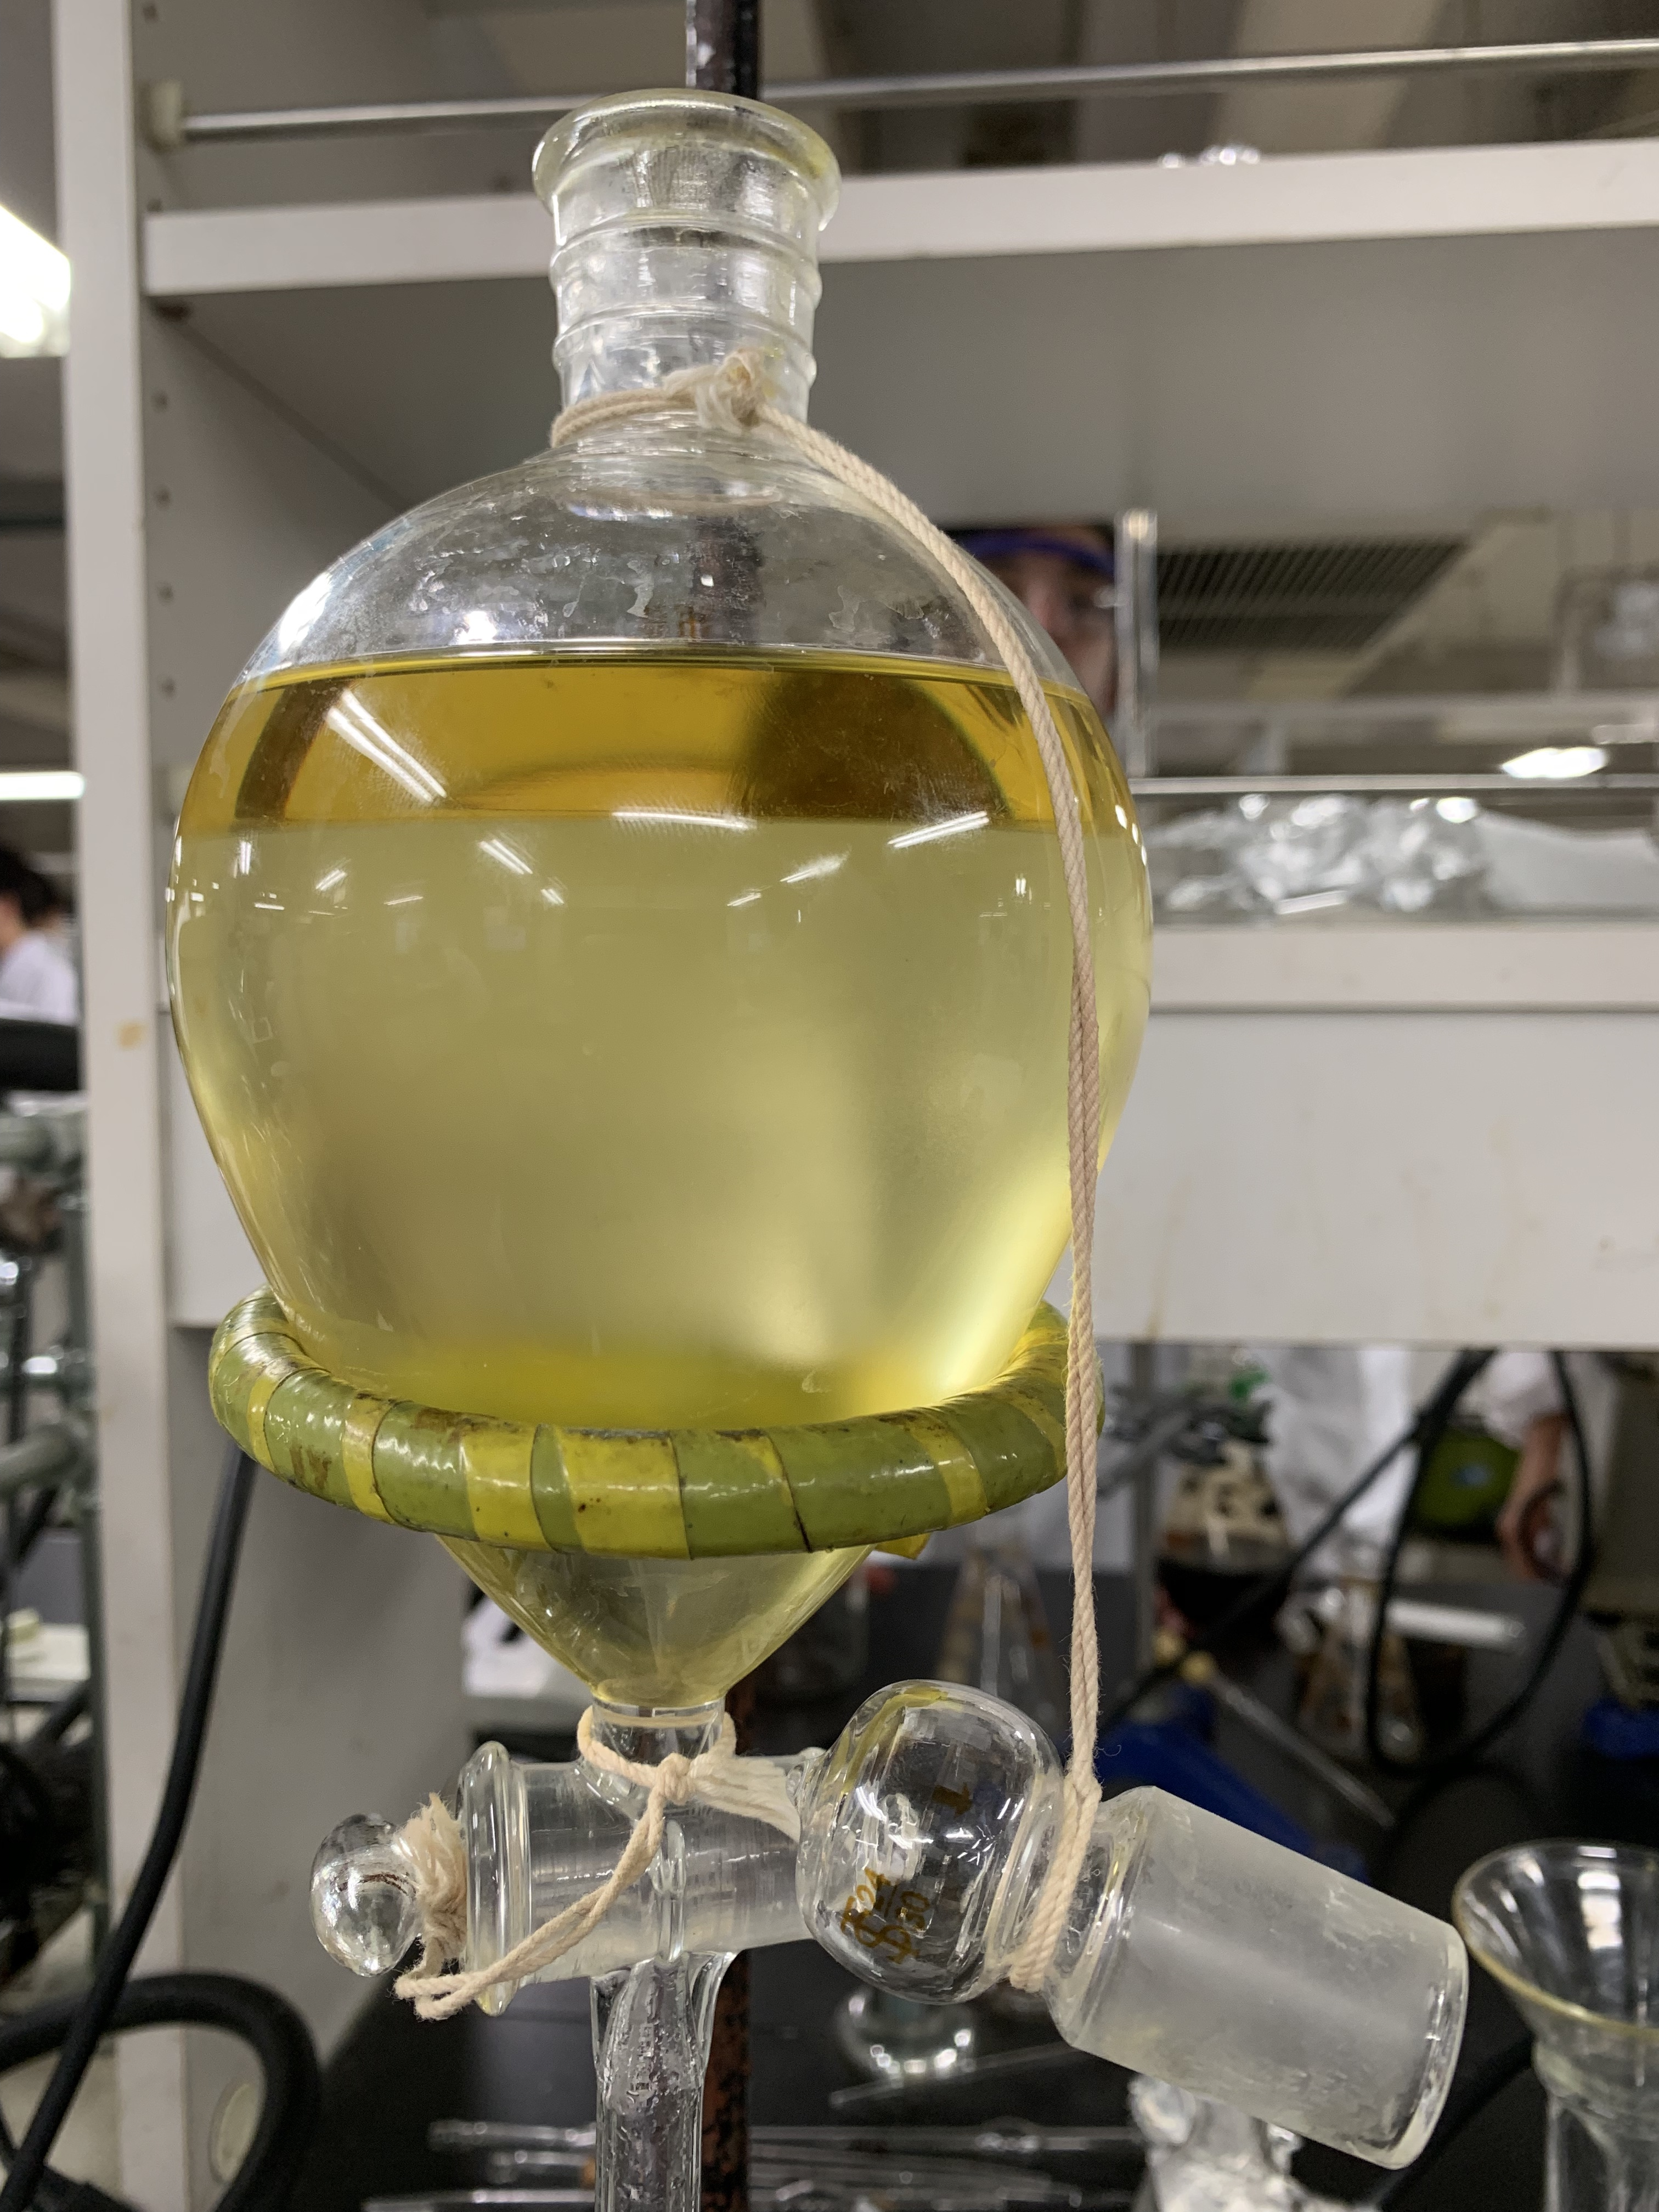
\includegraphics[clip, width=4cm]{imgs4/be3.jpg}
\hspace{1.6cm} 分液2回目
\end{center}
\end{minipage}

\begin{minipage}{0.05\hsize}
        \hspace{2mm}
      \end{minipage}

\begin{minipage}{0.20\hsize}
\begin{center}
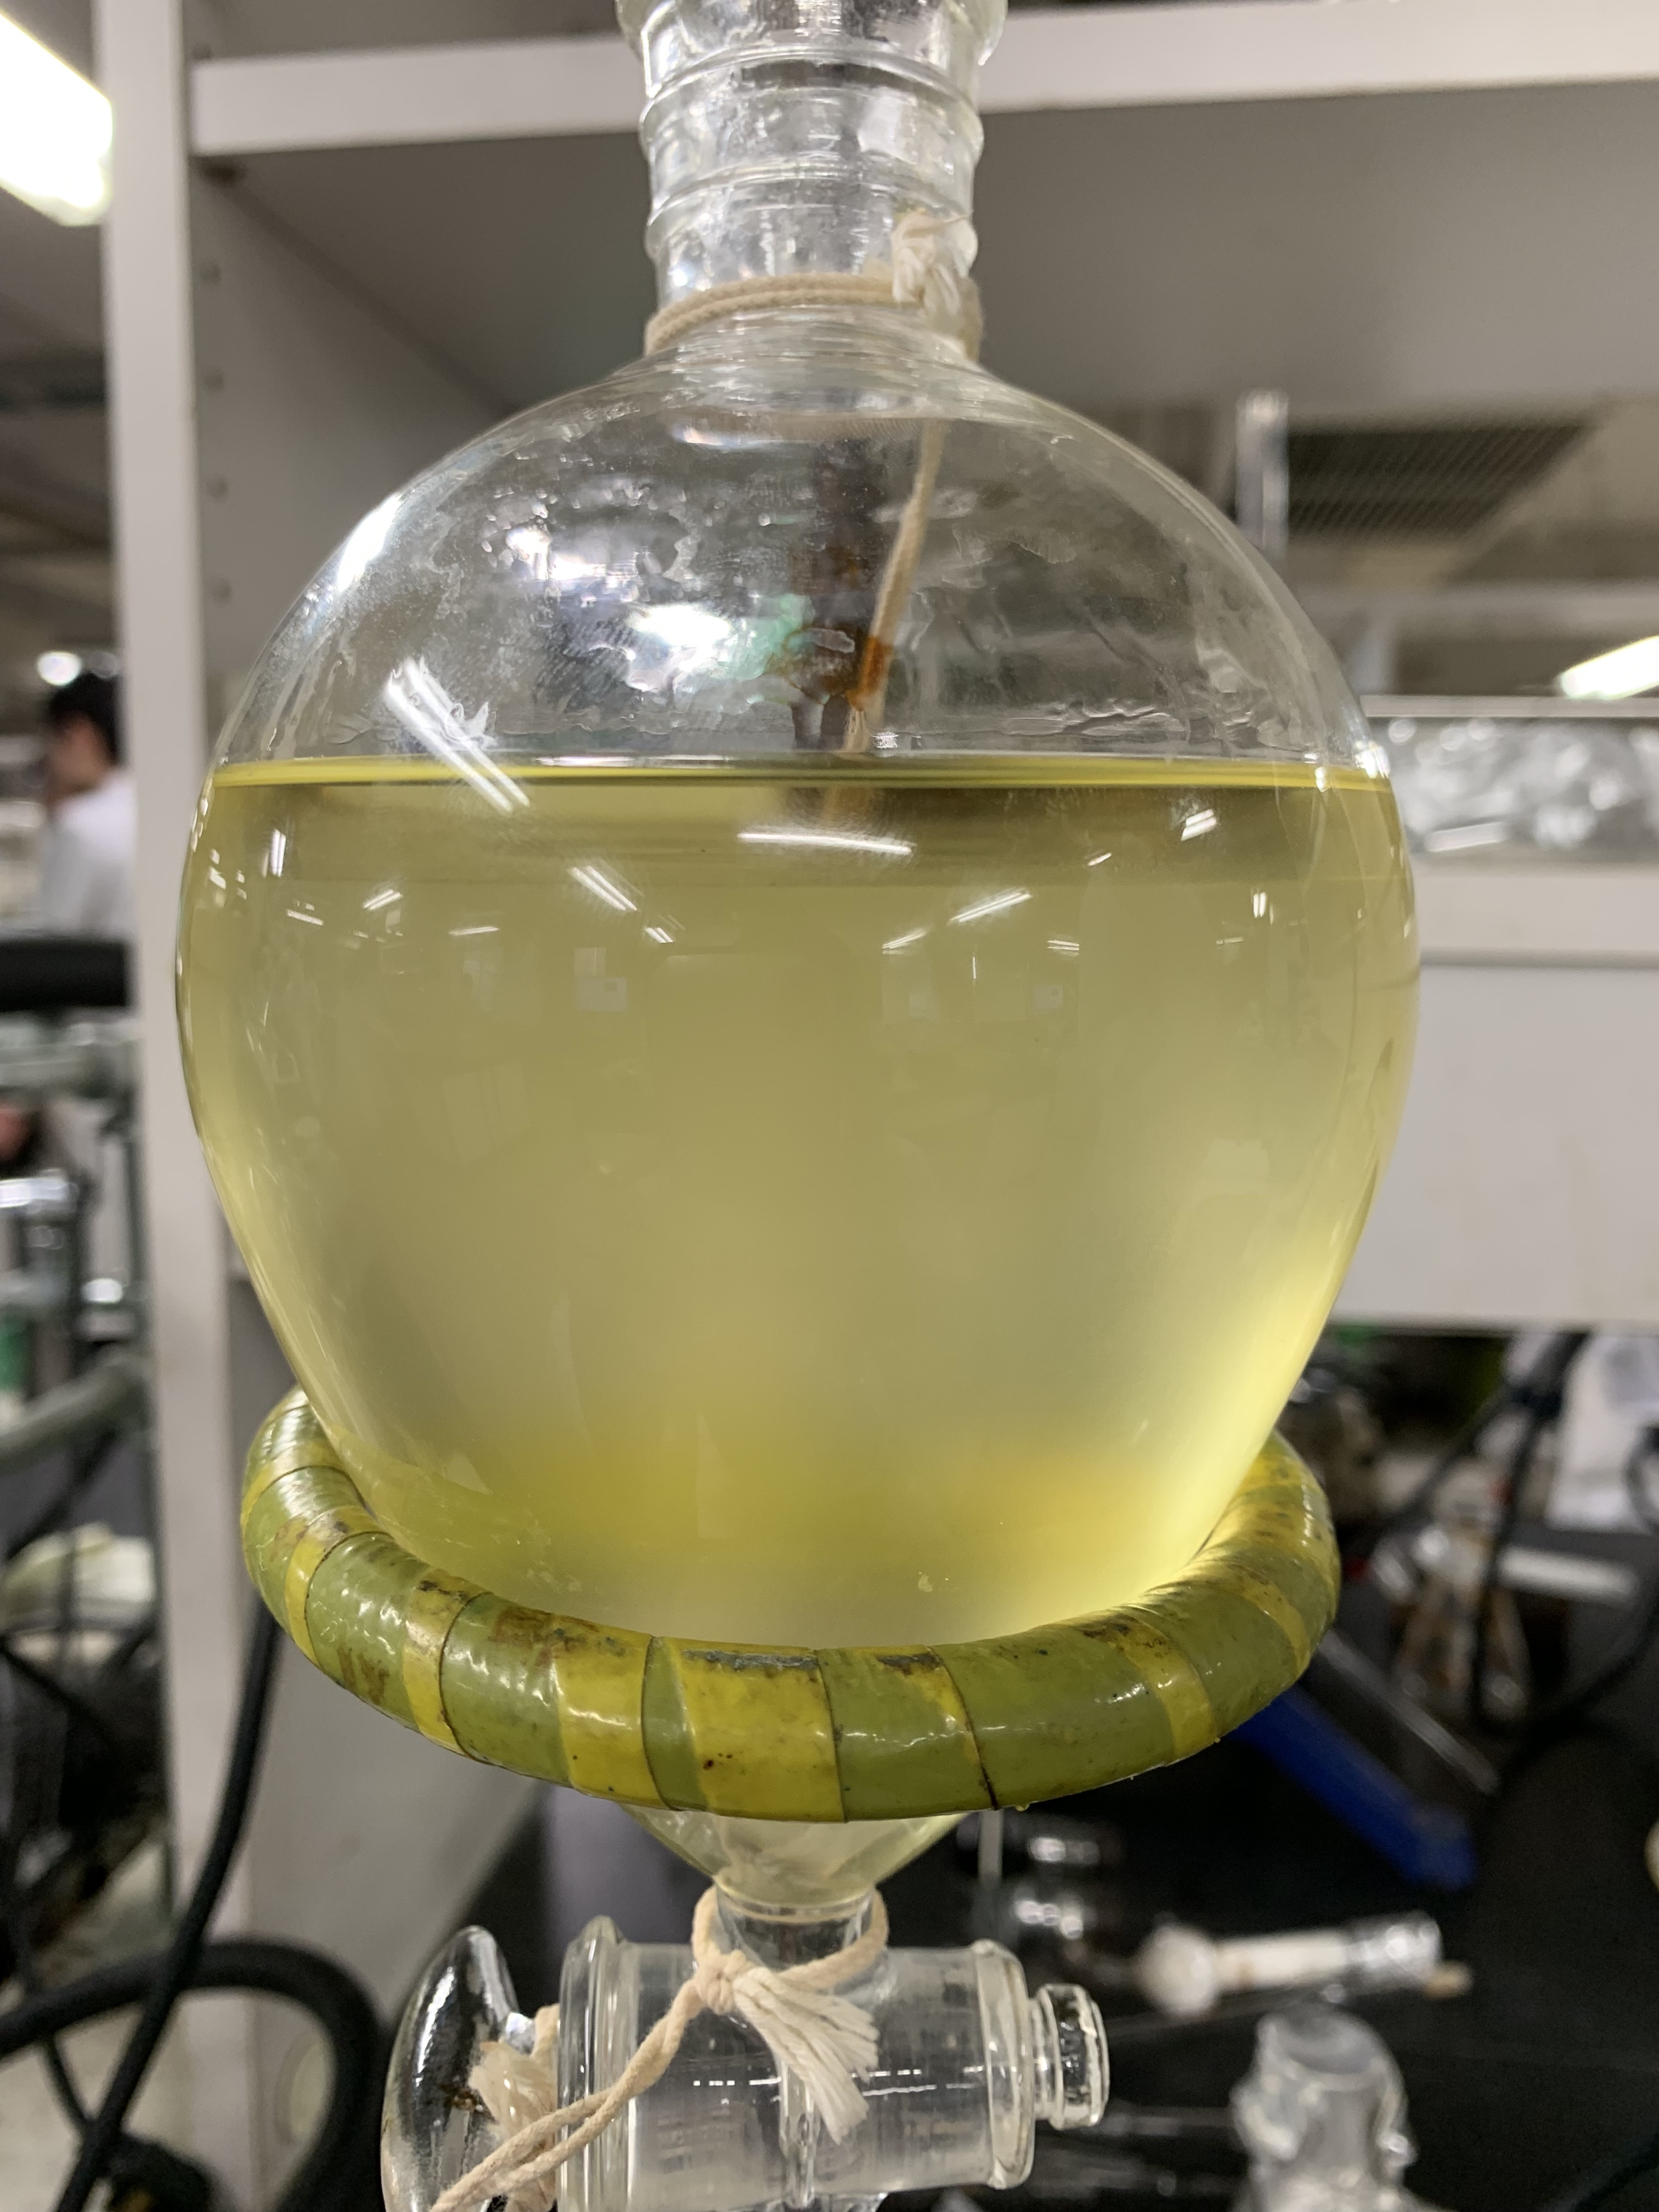
\includegraphics[clip, width=4cm]{imgs4/be4.jpg}
\hspace{1.6cm} 分液3回目
\end{center}
\end{minipage}

\end{tabular}
\end{center}
\end{figure}


\subsubsection*{TLC}


\begin{figure}[H]
\begin{center}
\begin{tabular}{c}

\begin{minipage}{0.20\hsize}
\begin{center}
\includegraphics[clip, height=6cm]{imgs4/tlc1.jpg}
\hspace{1.6cm} \footnotesize{30分 UV}
\end{center}
\end{minipage}

\begin{minipage}{0.05\hsize}
        \hspace{2mm}
      \end{minipage}

\begin{minipage}{0.20\hsize}
\begin{center}
\includegraphics[clip, height=6cm]{imgs4/tlc2.jpg}
\hspace{1.6cm} \footnotesize{30分 リンモリブデン酸}
\end{center}
\end{minipage}

\begin{minipage}{0.05\hsize}
        \hspace{2mm}
      \end{minipage}

\begin{minipage}{0.20\hsize}
\begin{center}
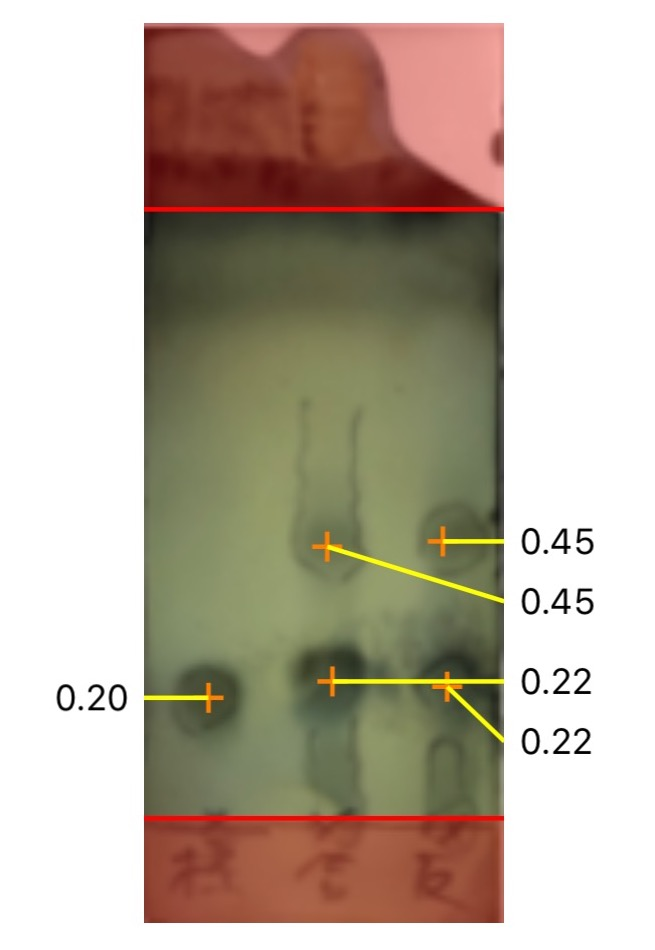
\includegraphics[clip, height=6cm]{imgs4/tlc3.jpg}
\hspace{1.6cm} \footnotesize{60分 UV}
\end{center}
\end{minipage}

\begin{minipage}{0.05\hsize}
        \hspace{2mm}
      \end{minipage}

\begin{minipage}{0.20\hsize}
\begin{center}
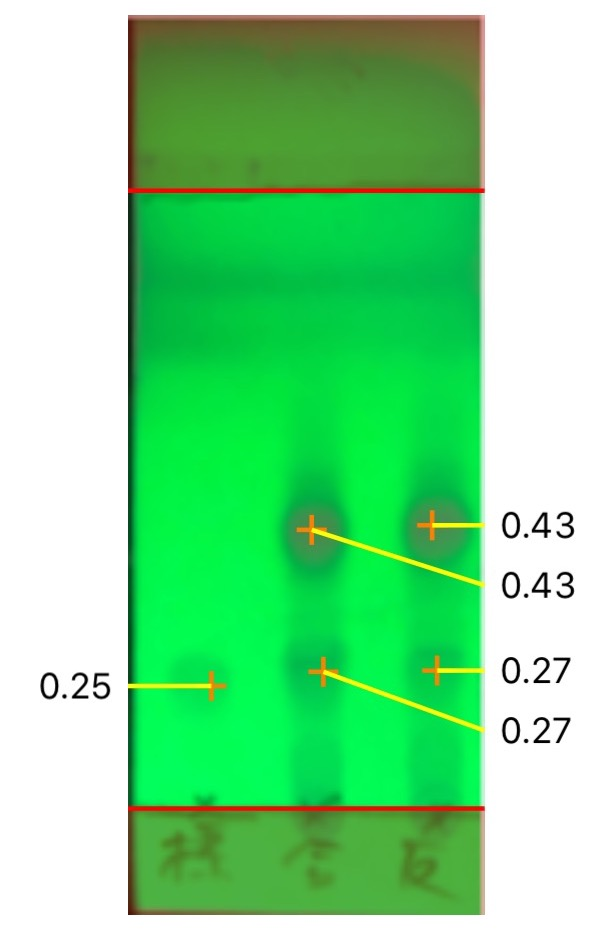
\includegraphics[clip, height=6cm]{imgs4/tlc4.jpg}
\hspace{1.6cm} \footnotesize{60分 リンモリブデン酸}
\end{center}
\end{minipage}

\end{tabular}
\end{center}
\end{figure}

\subsection*{考察}
抽出操作で極性が比較的強いAcOEtと極性が弱いetherを混合して使用したのは有機層にDMFをなるべく溶かしこまず、かつ有機層の極性をちょうど良い具合に調節するためである。

今回のTLCではメインのスポットの上下に帯状にスポットが広がっていた、これは反応で様々な副生成物ができていることを示している。

\section*{5日目 環拡大の精製}
\subsection*{結果}
\begin{itemize}
\item 3〜12分画を濃縮し、黄褐色の粉末状の結晶を得た。
\item 再結晶すると白と黄褐色が混ざった鱗片状の結晶が得られた。
\end{itemize}
\subsubsection*{再結晶}
\begin{itemize}
\item 重さ : 0.96 g
\item 収率 : 21.97 \%
\item 融点 : 142 ℃

\end{itemize}
\subsubsection*{TLC}


\begin{figure}[H]
\begin{center}
\begin{tabular}{c}

\begin{minipage}{0.15\hsize}
\begin{center}
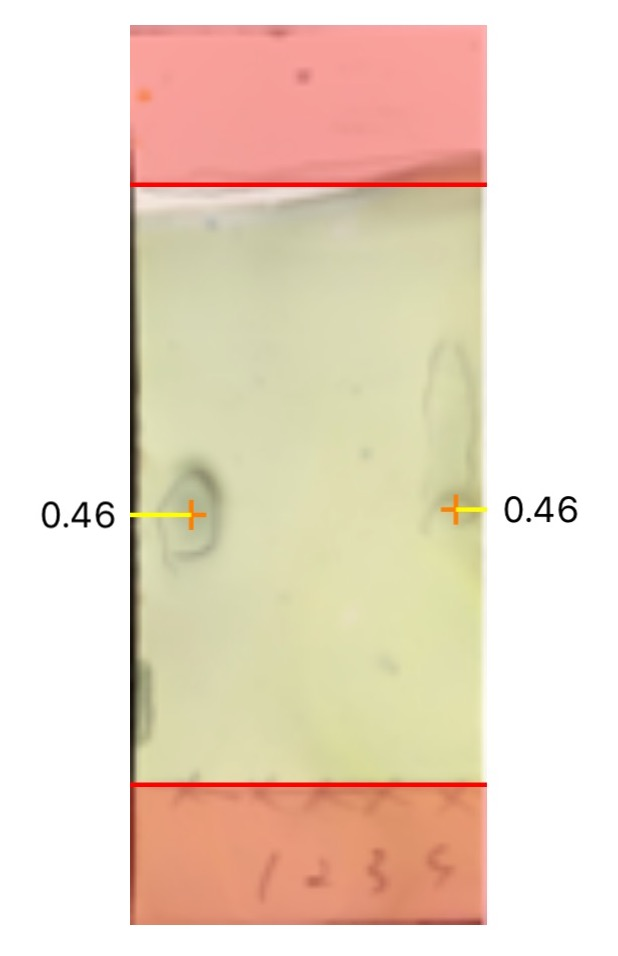
\includegraphics[clip, height=4cm]{imgs5/tlc-r1.jpg}
\hspace{1.6cm} 1〜4分画
\end{center}
\end{minipage}

\begin{minipage}{0.06\hsize}
        \hspace{2mm}
      \end{minipage}

\begin{minipage}{0.15\hsize}
\begin{center}
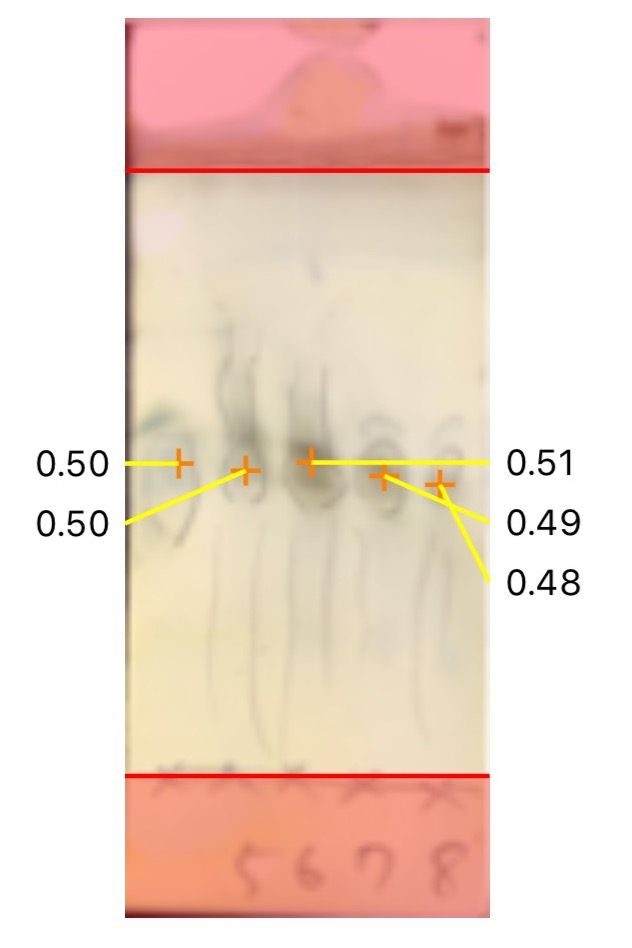
\includegraphics[clip, height=4cm]{imgs5/tlc-r2.jpg}
\hspace{1.6cm} 5〜8分画
\end{center}
\end{minipage}

\begin{minipage}{0.06\hsize}
        \hspace{2mm}
      \end{minipage}

\begin{minipage}{0.15\hsize}
\begin{center}
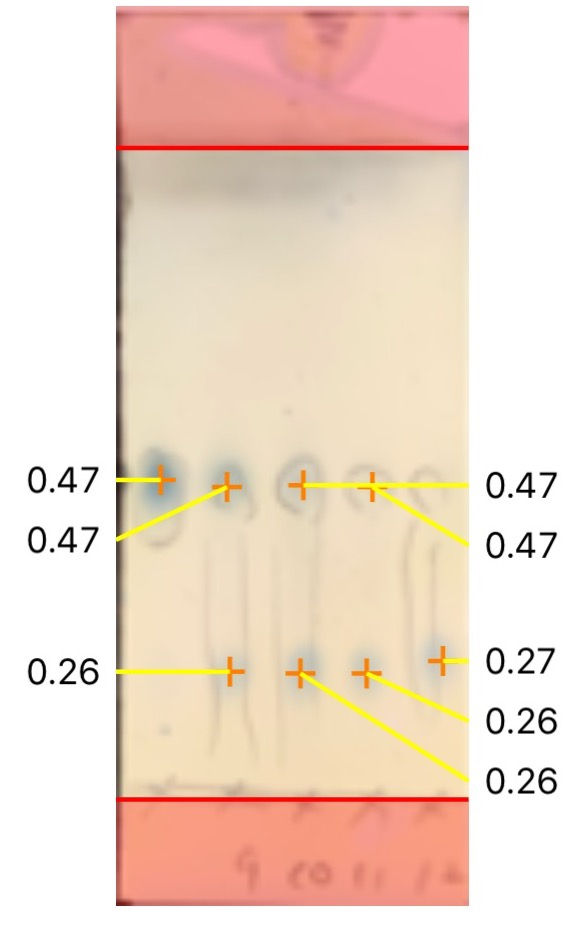
\includegraphics[clip, height=4cm]{imgs5/tlc-r3.jpg}
\hspace{1.6cm} 9〜12分画
\end{center}
\end{minipage}

\begin{minipage}{0.06\hsize}
        \hspace{2mm}
      \end{minipage}

\begin{minipage}{0.15\hsize}
\begin{center}
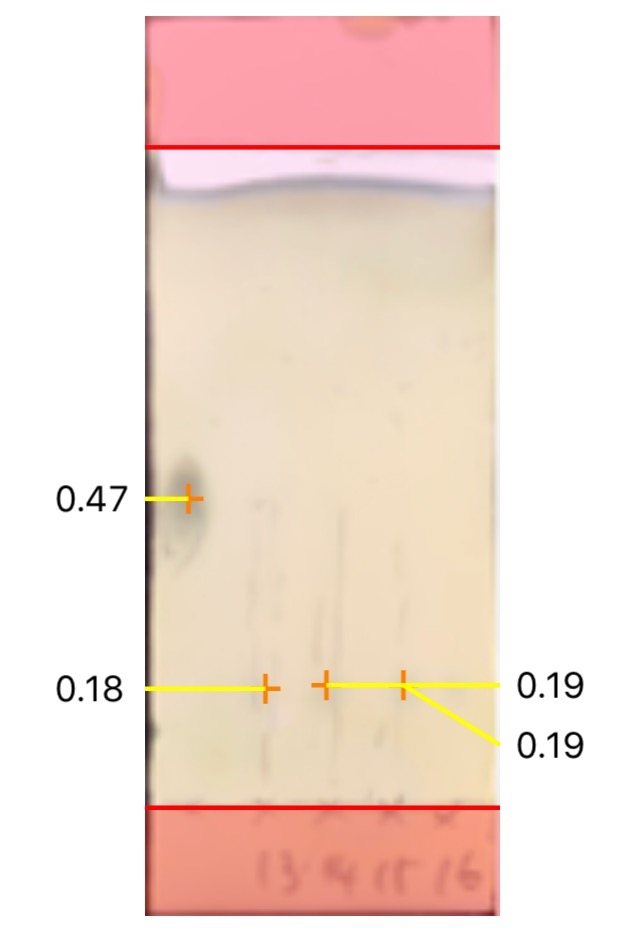
\includegraphics[clip, height=4cm]{imgs5/tlc-r4.jpg}
\hspace{1.6cm} 13〜16分画
\end{center}
\end{minipage}

\begin{minipage}{0.06\hsize}
        \hspace{2mm}
      \end{minipage}

\begin{minipage}{0.15\hsize}
\begin{center}
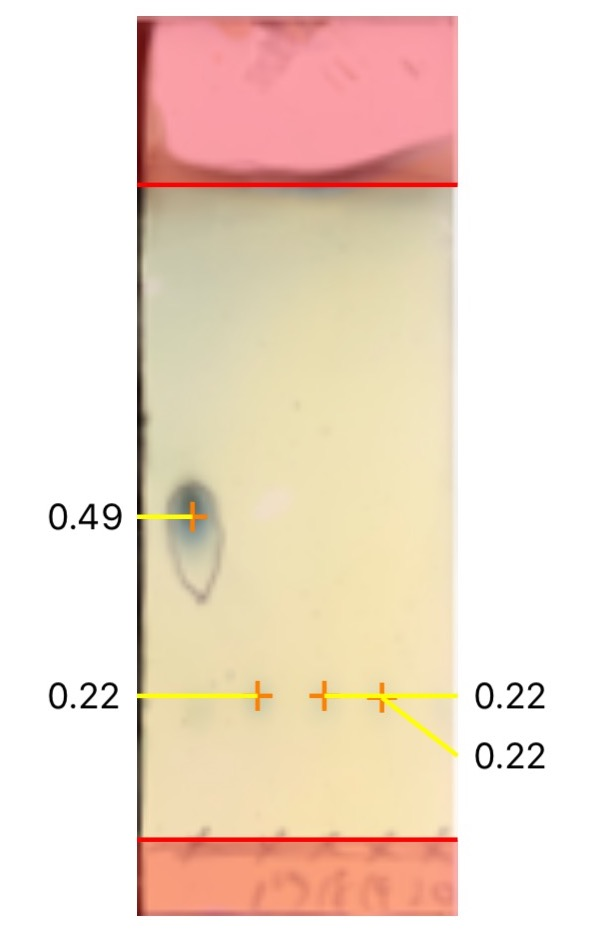
\includegraphics[clip, height=4cm]{imgs5/tlc-r5.jpg}
\hspace{1.6cm} 17〜20分画
\end{center}
\end{minipage}

\end{tabular}
\caption{リンモリブデン酸}
\end{center}
\end{figure}


\

\begin{figure}[H]
\begin{center}
\begin{tabular}{c}

\begin{minipage}{0.15\hsize}
\begin{center}
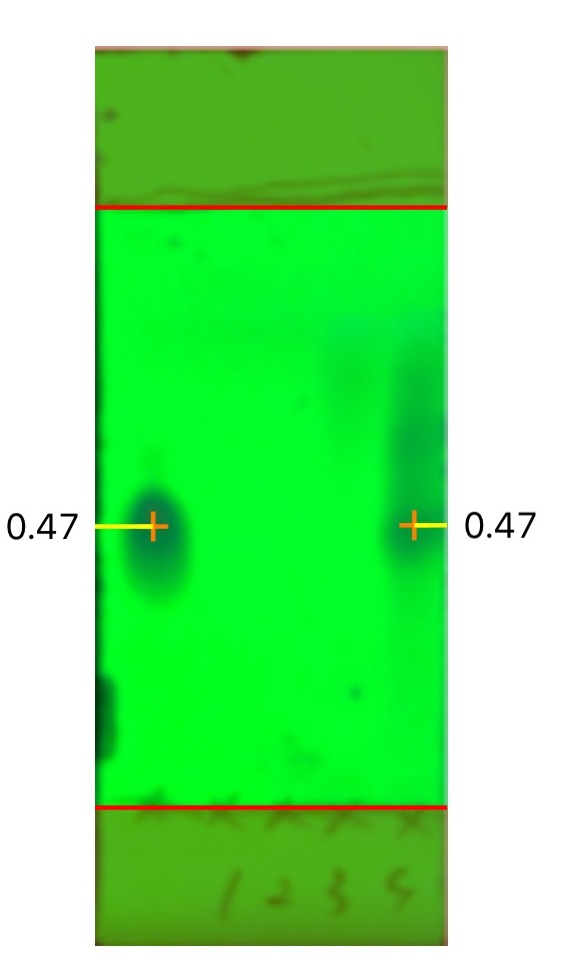
\includegraphics[clip, height=4cm]{imgs5/tlc-u1.jpg}
\hspace{1.6cm} 1〜4分画
\end{center}
\end{minipage}

\begin{minipage}{0.06\hsize}
        \hspace{2mm}
      \end{minipage}

\begin{minipage}{0.15\hsize}
\begin{center}
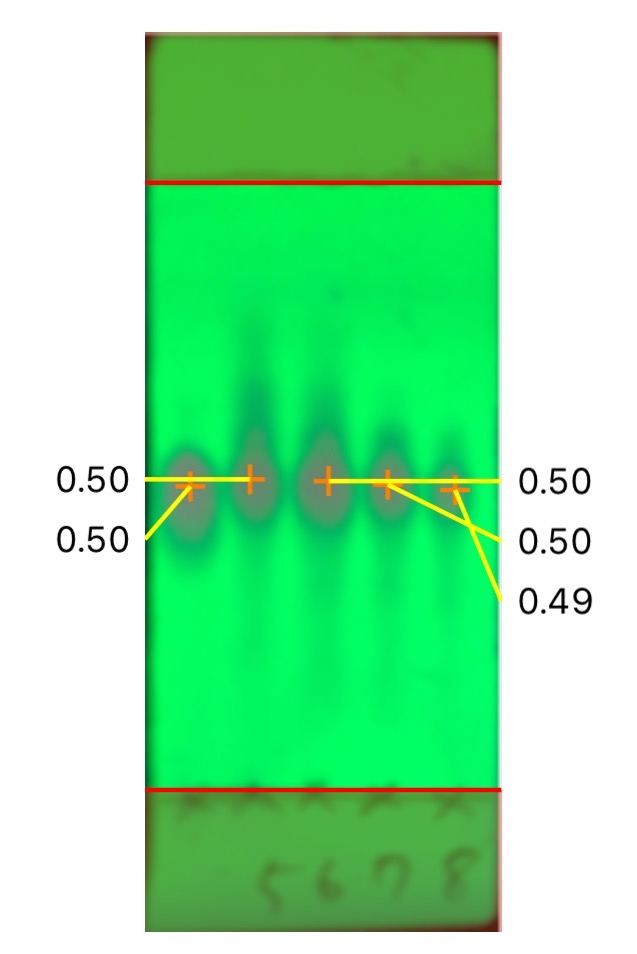
\includegraphics[clip, height=4cm]{imgs5/tlc-u2.jpg}
\hspace{1.6cm} 5〜8分画
\end{center}
\end{minipage}

\begin{minipage}{0.06\hsize}
        \hspace{2mm}
      \end{minipage}

\begin{minipage}{0.15\hsize}
\begin{center}
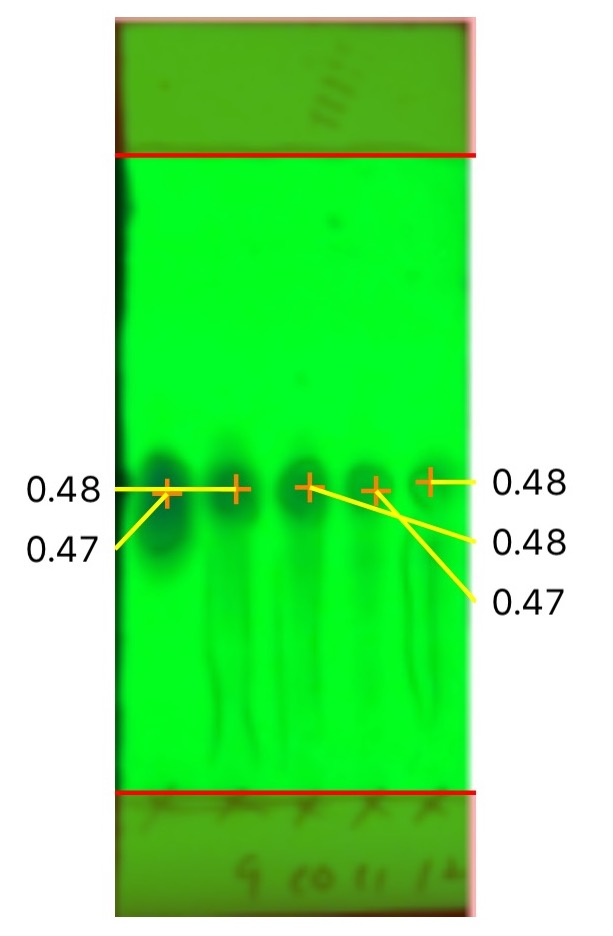
\includegraphics[clip, height=4cm]{imgs5/tlc-u3.jpg}
\hspace{1.6cm} 9〜12分画
\end{center}
\end{minipage}

\begin{minipage}{0.06\hsize}
        \hspace{2mm}
      \end{minipage}

\begin{minipage}{0.15\hsize}
\begin{center}
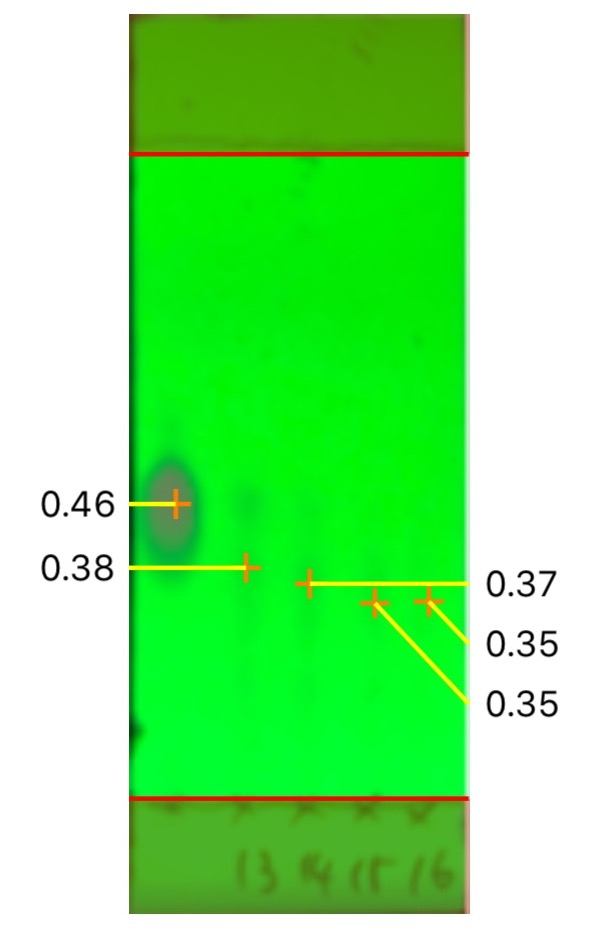
\includegraphics[clip,height=4cm]{imgs5/tlc-u4.jpg}
\hspace{1.6cm} 13〜16分画
\end{center}
\end{minipage}

\begin{minipage}{0.06\hsize}
        \hspace{2mm}
      \end{minipage}

\begin{minipage}{0.15\hsize}
\begin{center}
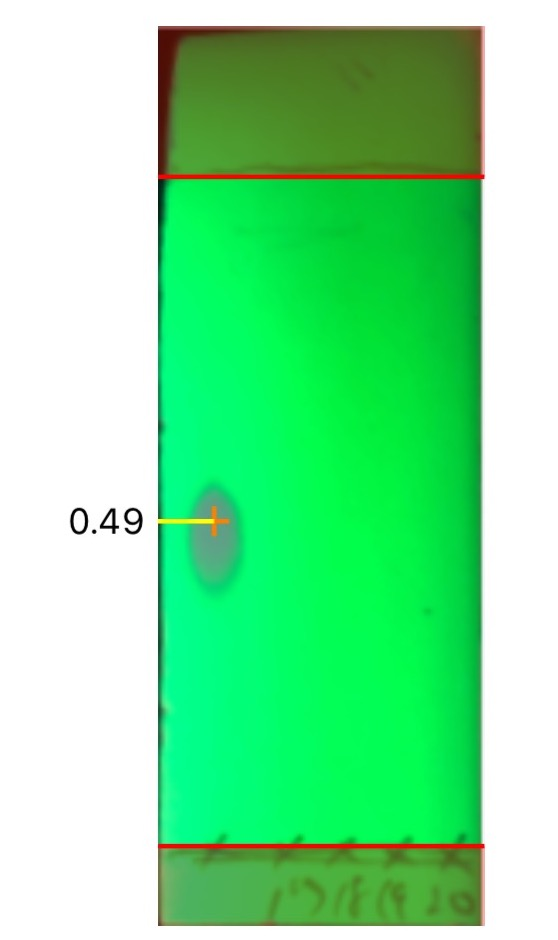
\includegraphics[clip, height=4cm]{imgs5/tlc-u5.jpg}
\hspace{1.6cm} 17〜20分画
\end{center}
\end{minipage}

\end{tabular}
\caption{UV}
\end{center}
\end{figure}



\section*{6日目 脱保護}
\subsection*{結果}
\begin{itemize}
\item 酢酸エチルと水を加えると白い結晶が大量に析出した。
\item 塩酸を加えると結晶が溶けていった。
\item エバポレーターで濃縮して白い結晶を得た。

\end{itemize}
\subsubsection*{再結晶}
\begin{itemize}
\item 重さ : 0.03 g
\item 収率 4.36 \%
\item 融点 : 169 ℃

\end{itemize}


\section*{課題}

\begin{tcolorbox}[colback=white,colbacktitle=black,coltitle=white,title={1-a.}]
トリクロロエチルエステル化の反応機構を記せ。
\end{tcolorbox}

\pict{imgs-k/hk1.jpeg}{10}
\pict{imgs-k/hk2.jpeg}{10}
求核性および脱離能の高いピリジンが触媒として働いている。

\begin{tcolorbox}[colback=white,colbacktitle=black,coltitle=white,title={1-b.}]
トリクロロエチルエステルとして保護する理由を述べよ。他の考えられる代表的なカルボン酸の保護基を挙げつつ、それぞれのケースで考えられる問題点と照らしながら説明すること。
\end{tcolorbox}

代表的なカルボン酸の保護としては酸を用いたエステル化や縮合剤を用いた手法が考えられる。しかし過剰な酸性条件にするとラクタム環が壊れてしまうためエステル化による保護はできない。また、DCCなどの縮合剤を用いた場合は生成物と同量の不要な化合物が生じてしまい、それを取り除くのにカラムクロマトグラフィーをする必要がある。そのコストを減少させるために今回はTroc基による保護を行った。

\begin{tcolorbox}[colback=white,colbacktitle=black,coltitle=white,title={1-c.}]
スルホキシド体の酸化において、$\beta -$スルホキシド基が選択的に得られる理由を述べよ。またアミノ基の保護基としてフタルイミドを用いた場合の結果を予想せよ。
\end{tcolorbox}


今回のスルホキシドの形成反応では硫黄原子が過ギ酸の酸素原子を攻撃することで形成されるが、この反応はより混み合っているconcave面での反応を経由して$\beta$スルホキシドを形成するが、これはconcave面を経由することで図に示すような水素結合による安定化が起こり、concaveの立体障害による不利をうち系していると考えられる。
そのためアミンを部分をフタルイミドで保護するとそのような結合が形成されないと考えられるので、立体的にあまり混み合っていないconvex面から反応が進行して光学異性体のスルホキシドが形成される。

\pict{imgs-k/1c.jpeg}{5}

\begin{tcolorbox}[colback=white,colbacktitle=black,coltitle=white,title={1-d.}]
環拡大反応の反応機構を記せ。カルボキシ基を保護しないで行った場合、どのような問題点が考えられるか。
\end{tcolorbox}

\pict{imgs-k/hk-1d.jpeg}{10}
カルボキシ基を保護しないと無水酢酸と反応してエステルを形成すると考えられる。

\begin{tcolorbox}[colback=white,colbacktitle=black,coltitle=white,title={1-e.}]
トリクロロエチルエステル脱保護の反応機構を示せ。
\end{tcolorbox}

\pict{imgs-k/hk-1e.jpeg}{10}


\begin{tcolorbox}[colback=white,colbacktitle=black,coltitle=white,title={2.}]
NMR・IRのスペクトルピークを帰属せよ。
\end{tcolorbox}


\subsubsection*{化合物A}
\begin{itemize}
\item セファロスポリン

ハロゲンエステルを特徴付ける$\delta = 4 \sim 4.5$のピークがないのが特徴である。
\end{itemize}

\subsubsection*{化合物B}

\begin{itemize}
\item 環拡大体

六員環があるのでメチル基の化学シフトが小さい。

\end{itemize}

\subsubsection*{化合物C}
\begin{itemize}
\item S-Oxide体

分子内の電位の偏りによって水素の化学シフトが小さくなる。
\end{itemize}

\subsubsection*{化合物D}
\begin{itemize}
\item トリクロロエチルエステル体

消去法で求めた。
\end{itemize}












\begin{tcolorbox}[colback=white,colbacktitle=black,coltitle=white,title={3.}]
細菌の細胞壁合成経路を概説し、$\beta -$ラクタム系抗生物質とバンコマイシンの作用機序について構造式を使いながらそれぞれ簡単に説明せよ。
\end{tcolorbox}

細菌の細胞壁の構成成分はグラム陰性かグラム陽性かで異なる。しかしほとんどの細菌はペプチドグリカンという糖ペプチドの重合体を構成要素に持っている。ペプチドグリカン合成は細菌類に特異的なのでこの反応を標的とした抗生物質は多く、ペニシリンやバンコマイシンもその一種である。

ペプチドグリカン合成は以下の3つの順序で行われる
\begin{enumerate}
\item UDP-MurNAc-ペンタペプチド合成
\item ムレインモノマーの合成
\item ペプチドグリカンの伸長

\end{enumerate}
\subsubsection*{UDP-MurNAc-ペンタペプチド合成}
\pict{imgs-k/k3-1.jpg}{14}

このステップを阻害する抗生物質はバンコマイシンやシクロセリンなどである。

\subsubsection*{ムレインモノマーの合成}
ムレインモノマーの合成は以下の4段階からなる。リピドピロリン酸などの抗生物質がこのステップを阻害する。
\begin{enumerate}
\item ペンタペプチドのリン酸を介した脂質担体との結合
\item GluNAc-UDPを介したMurNAcとGluNAcの結合
\item t-RNAを介したグリシンのL-Lys or m-Dpmに対する結合
\item リピド担体による細胞外への運搬およびリピドからアクセプターへの転移
\end{enumerate}


\subsubsection*{ペプチドグリカンの伸長}
ペプチドグリカンの伸長は以下の3段階からなる。
\begin{enumerate}
\item D-Alaの脱離に伴うペンタグリシンによる架橋形成
\item もう一方のD-Ala脱離
\item MurNAcとGluNAc部の結合形成

特に重要なのが1番目のreanspeptidationの過程であり、ペニシリンやセファロスポリンの作用点である。これらを総称して$\beta$ラクタム系抗生物質という。

\end{enumerate}
\subsubsection*{バンコマイシン}
\pict{imgs-k/bkm.png}{10}
バンコマイシンは巨大な塩基性配糖体であり、細胞内のUDP-MurNAc-ペンタペプチドのD-Ala-D-Ala末端に水素結合を介して結合することで、細菌類のペプチドグリカン合成を阻害している。
ただしその非常に大きな分子量であるがゆえにグラム陰性菌の細胞壁を通過することができず、効果があるのはグラム陽性菌に限られる。しかし、多剤耐性菌であるMRSAにも効果を発揮するので医療現場においては非常によく用いられている。

\subsubsection*{$\beta$ラクタム系抗生物質}
\pict{imgs-k/btr.png}{6}
ペニシリン類をはじめとする$\beta$ラクタム系抗生物質はペプチドグリカンのD-Ala-D-Ala様の構造をとっており、この部分を基質とするペプチドグリカントランスペプチターゼを競争的に阻害している。$\beta$ラクタム系抗生物質は作用点が細胞外部であり、抗菌スペクトルが多く静菌的ではなく殺菌的に作用するので臨床的利用も多いが耐性菌の存在が問題となっている。

\begin{tcolorbox}[colback=white,colbacktitle=black,coltitle=white,title={4.}]
$\beta -$ラクタム系抗生物質とバンコマイシンに対する細菌の耐性獲得機構を、構造式を用いながらそれぞれ説明せよ。
\end{tcolorbox}


\subsubsection*{$\beta -$ラクタム系抗生物質に対する耐性の獲得}
\pict{imgs-k/rktm.jpg}{10}
ペニシリンなどの$\beta$ラクタム環を破壊する$\beta$-ラクタマーゼやアミドを分解するペニシリンアシダーゼなどの酵素タンパクをコードする耐性菌が現れたことが問題となった。科学者はペニシリナーゼが効かないカルバペネム系などの抗生物質を開発するが、細菌も新たな酵素を獲得して耐性菌が生まれるといういたちごっこを繰り返している。


\subsubsection*{バンコマイシンに対する耐性の獲得}
\pict{imgs-k/tsk.png}{10}
赤色の分子がバンコマイシンを表し、緑色の部分が細菌の細胞壁合成に必要なムレインモノマーの、結合部分を表している。バンコマイシンは、水色の点線で現したように、5本の水素結合で強固に結びついて、細胞壁の合成を阻害するが、バンコマイシン耐性菌では、ムレインモノマーの構造が矢印で示すように、一部変化ているために、バンコマイシンが水素結合できなくなっている。その結果バンコマイシンが細胞壁の合成を阻害できなくなり、抗菌力を失ってしまう。

\begin{tcolorbox}[colback=white,colbacktitle=black,coltitle=white,title={5.}]
新規反応開発研究が医薬プロセス化学にどのようなインパクトを与えるか、またこれによって世界はどのように良くなっていくかについて、考察せよ。
\end{tcolorbox}


医薬品の開発において経済的に大量生産するためのプロセス化学は新たな薬を開発する創薬化学と両輪になって前に進んでいくものである。工業化に伴う経済性や安全性、法律といった課題を考慮しながら薬を世に送り出す非常に重要な学問であると言える。したがって新規反応開発研究によってもたらされる学問の進歩、経済効果は計り知れない。安定した薬の供給を実現することによって、世界中の今まで薬に手が届かなかった人々に薬が行き届く日が実現するだろう。




\end{document}
